%!TEX root = ../terrainbook.tex

\graphicspath{{mat/}}
\label{chap:mat}

\chapter{The medial axis transform}

% \section{Introduction} % what is it, how defined, why useful+examples of applications
Until now, we have described the shape of a terrain using the boundary representation. 
The boundary representation, or \emph{b-rep}, is the most commonly used shape representation for DTMs, \ie\ we model a terrain by describing explicitly its boundary surface, \eg\ using points, grid cells, triangles, or contour lines.
The medial axis transform (MAT) gives us another way to represent shape.
Contrary to the B-rep, the MAT describes a shape by its skeleton instead of its boundary (compare Figures~\ref{fig:gbm:brep} and \ref{fig:gbm:maxis}).
\begin{figure}[tbp]
	\centering
	\begin{subfigure}[b]{0.25\linewidth}
		\centering
		
\includegraphics[width=\textwidth]{figs/gingerbreadman_whole.pdf}
		\caption{A 2D object}
		\label{fig:gbm:whole}
	\end{subfigure}
	\qquad%
	\begin{subfigure}[b]{0.25\linewidth}
		\centering
		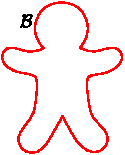
\includegraphics[width=\textwidth]{figs/gingerbreadman_brep.pdf}
		\caption{B-rep}
		\label{fig:gbm:brep}
	\end{subfigure}
	\qquad%
	\begin{subfigure}[b]{0.25\linewidth}
		\centering
		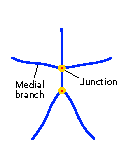
\includegraphics[width=\textwidth]{figs/gingerbreadman_skeleton.pdf}
		\caption{Interior MAT}
		\label{fig:gbm:maxis}
	\end{subfigure}

	\begin{subfigure}[b]{0.3\linewidth}
		\centering
		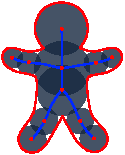
\includegraphics[width=\textwidth]{figs/gingerbreadman_mat.pdf}
		\caption{Medial balls}
		\label{fig:gbm:mballs}
	\end{subfigure}
	\qquad
	\begin{subfigure}[b]{0.3\linewidth}
		\centering
		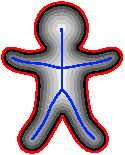
\includegraphics[width=\textwidth]{figs/gingerbreadman_grassfire.pdf}
		\caption{Contours of equal distance to the boundary.}
		\label{fig:gbm:dt}
	\end{subfigure}

	\caption{Different ways to represent the shape of gingerbread man}
	\label{fig:gingerman}
\end{figure}

The MAT can be considered a \emph{dual} representation to the B-rep, similar to how the Voronoi diagram is dual to the Delaunay triangulation. 
Both the MAT and the B-rep contain exactly the same information and it is possible to convert one to the other without loss of information.
However, the two different representations expose different properties of a shape which means they both have their own unique use cases. 
% information is represented differently and both representations have different properties.
%  and in certain cases---it depends on what you are aiming to do---one is much more useful than the other.

For example, the MAT allows us to split a shape into parts simply by looking at the branches of the skeleton. 
The resulting shape parts often turn out to be meaningful in practice. 
Observe for instance that for the gingerbread man in Figure~\ref{fig:gingerman}, its arms, legs, torso and head each have one corresponding branch in its medial axis (compare Figures~\ref{fig:gbm:whole} and \ref{fig:gbm:maxis}).
For DTMs, equally meaningful decompositions into parts can be made, \eg\ the MAT allows us to decompose a DTM into separate hills, watercourses and other objects on top the DTM (see Figure~\ref{fig:matterrain}).
\begin{figure}[tbp]
	\centering
	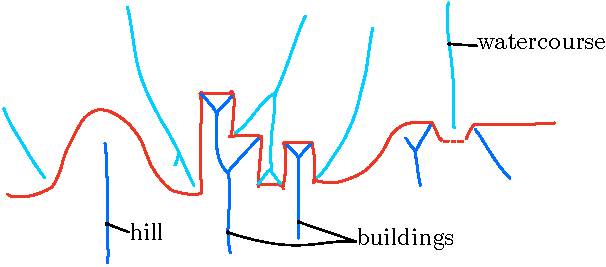
\includegraphics[width=0.8\linewidth]{figs/MAT_hierarchy.pdf}
	\caption{For a terrain the MAT is typically subdivided into open clusters that correspond to features such as hills, buildings and watercourses in the terrain. Shown here is a vertical cross section of a DTM. Exterior MAT in light blue, interior MAT in dark blue.}
	\label{fig:matterrain}
\end{figure}

In the context of DTMs both the 2D and the 3D MAT are used. 
The 2D MAT is used for operations on sets of 2D curves, such as isolines or river networks. 
In these cases no elevation information is used to construct the MAT.
With the 3D MAT on the other hand, the whole surface of the terrain, including the elevation, is used during construction.
% because the MAT contains the same information, but models key properties of a shape in a more intuitive and explicit way.
% The key benefit of the MAT here is its skeleton-like representation that explicitly encodes the structure of a shape through a set of connected \emph{medial sheets}.
% At the same time it also encodes the full geometry of a shape as the union of its medial balls that effectively describes the volume of the shape.

% For example, in this thesis I demonstrate that a point cloud can be decomposed in meaningful parts such as separate buildings, by using a decomposition of the MAT.
% The MAT brings us a new perspective in point cloud modelling and the underlying hypothesis of this thesis is that certain operations on point clouds can be achieved more effectively by using its MAT, rather than its surface points directly.

% In particular, the MAT gives us 1) an elegant way to structure and decompose a point cloud into meaningful objects such as buildings and watercourses in a geographical scene, 2) an explicit separation into interior and exterior volumes in the point cloud, and 3) the local medial geometry: a set of measures to characterise shapes. 

\section{Defining the MAT}
There are two equivalent definitions of the MAT\footnote{Sometimes the MAT is referred to as medial axis function, stick figure, skeleton or surface skeleton.
Inventor Harry Blum finally settled on symmetry axis, as he considered symmetry to be the crucial role of the MAT \citep{Blum73}.}. 
One is based on the distance transform, and one is based on medial balls. 
Both definitions describe how to obtain the MAT from the boundary, denoted $
\mathcal{B}$ of an object (Figure~\ref{fig:gbm:brep}). 
And both can be applied to both 2D and 3D shapes.

\begin{description}
\item[Grassfire analogy]
Imagine that everything is made of grass and that all the points on $\mathcal{B}$ are simultaneously set on fire at time $t=0$. 
The fire spreads evenly to all directions at constant speed. 
Now, the MAT is defined as the set of points where the fire front meets itself. 
This concept is illustrated in Figure~\ref{fig:gbm:dt}, where each contour can be seen as a fire front at some constant time $t$. The medial axis is drawn where the fire front meets itself.
\item[Medial balls]
A \emph{medial ball} is a ball that fits completely inside $\mathcal{B}$ and does not contain any other ball that would fit inside $\mathcal{B}$. 
The MAT is defined as the set of points that are the centres of all medial balls of $\mathcal{B}$ (see Figure~\ref{fig:gbm:mballs}). 
Notice that each medial ball touches $\mathcal{B}$ in at least two points, called its \emph{feature points}. 
\end{description}

%TODO: that should also be in the figure
As illustrated in Figure~\ref{fig:gbm:maxis}, the MAT can be subdivided into \emph{medial branches} and \emph{junctions}. 
Junctions are locations where three or more medial branches coincide. 
The points of the MAT are called \emph{medial atoms}, or simply \emph{atoms}. 
Observe that if an atom has exactly two feature points, it is part of a medial branch, and if it has more than two feature points it lies on a junction or on the tip of a medial branch. 
The medial branches, its junctions and how those are are connected define the \emph{medial structure}.
% If we consider that each branch corresponds to one part of $\mathcal{B}$ gives us a natural way to split an object into parts

For a 2D object, such as in Figure~\ref{fig:gingerman}, the medial branches are curves and the the junctions are points. 
However, for a 3D object, the medial branches can also be surfaces (see Figure~\ref{fig:amentahand}), and the junctions can also be curves.
\begin{figure}[bp]
	\centering
	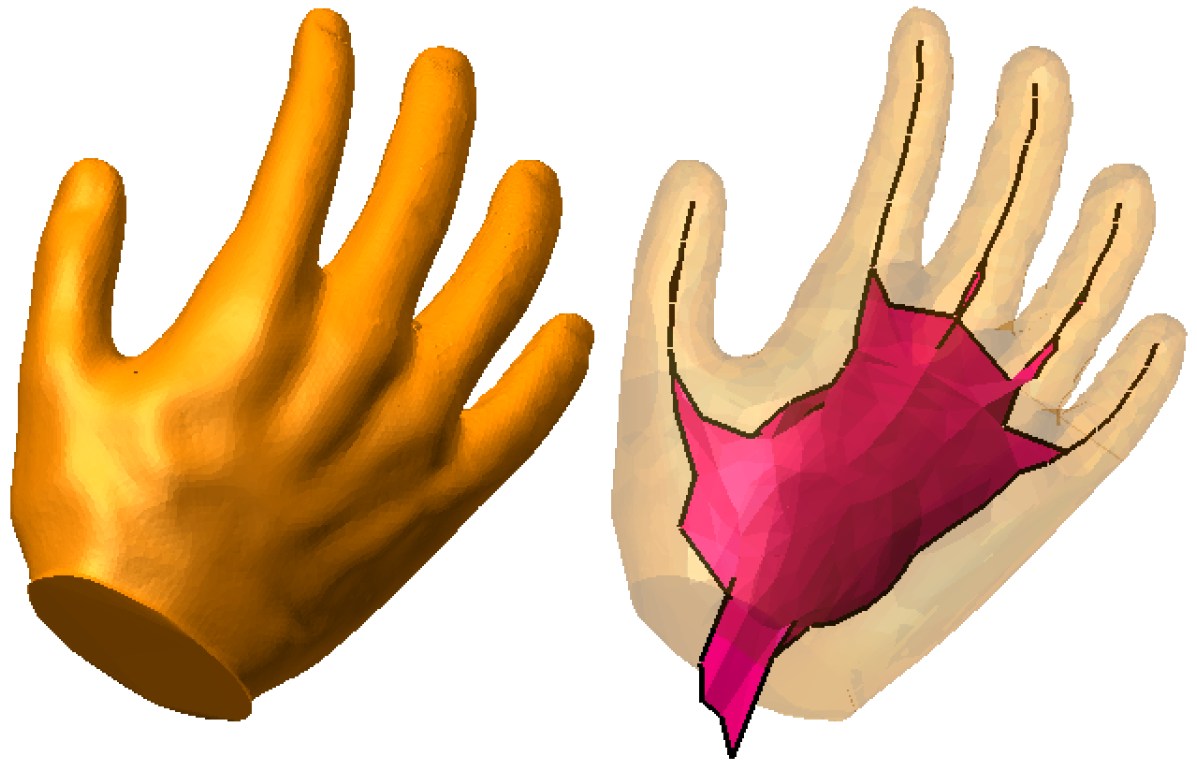
\includegraphics[width=0.6\linewidth]{figs/amenta_hand.png}
	\caption{An example of the 3D MAT \citep{Amenta01pc}.}
	\label{fig:amentahand}
\end{figure}
The branches of the 3D MAT are therefore also called \emph{medial sheets}.

\subsection{Medial geometry}
The medial geometry describes how atoms are related to the object boundary $\mathcal{B}$. 
It is defined for each medial atom that is part of a medial sheet. 
Figure~\ref{fig:medialgeometry} illustrates the complete medial geometry of an atom.
The medial ball $B$ has the atom $\mathbf{c}$ at its center and has a radius $r$, \ie\ the shortest distance from $\mathbf{c}$ to $\mathcal{B}$.
The medial ball $B$ touches the boundary $\mathcal{B}$ at the feature points $\mathbf{p}$ and $\mathbf{q}$.
The vectors from $\mathbf{c}$ to $\mathbf{p}$ and $\mathbf{q}$ are called the \emph{spoke vectors}, denoted $\vec{\mathbf{s_{p}}}$ and $\vec{\mathbf{s_{q}}}$. 
The angle between the spoke vectors is called the \emph{separation angle}, denoted $\theta$ and the bisector of the spoke vectors is called the \emph{medial bisector}, denoted $\vec{\mathbf{b}}$.

\begin{figure}[tbp]
	% \centering
	% \setcapindent{1em}
	\centering
	\begin{minipage}[c]{0.4\linewidth}
		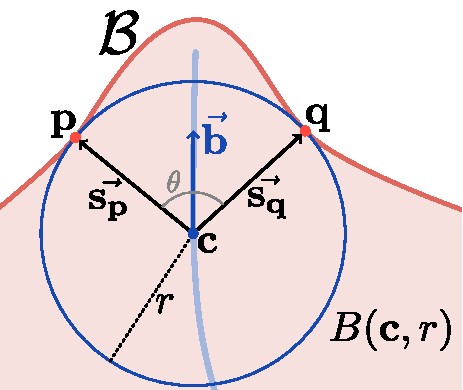
\includegraphics[width=\linewidth]{figs/medial_atom_geometry.pdf}
	\end{minipage}
	\begin{minipage}[c]{0.45\textwidth}
		% \hspace{1.1em}
		\centering
		\begin{tabular}{ll}
			\toprule
			Symbol & Description \\
			\midrule
			$B(\mathbf{c},r)$& medial ball\\
			$\mathbf{c}$ & medial atom\\
			$r$ & radius\\
			$\mathbf{p}, \mathbf{q}$ & feature points\\
			$\vec{\mathbf{s_{p}}}, \vec{\mathbf{s_{q}}}$ & spoke vectors\\
			$\theta$ & separation angle\\
			$\vec{\mathbf{b}}$ & medial bisector\\
			\bottomrule
		\end{tabular}
	\end{minipage}
	\caption{The geometry of a medial atom.}
	\label{fig:medialgeometry}
\end{figure}

% maximal/medial ball, primary and secondary feature point, primary and secondary medial ball, separation angle, bisector, medial atom:point+ball+metrics, 
% defining local coordinate system
% \subsection{Properties of the MAT}
Using the medial geometry we can describe a number of interesting properties of the MAT.
\begin{enumerate}
	\item Any atom $\mathbf{c}$ is always \emph{medial} to $\mathcal{B}$, \ie\ it is equidistant to the feature points of $\mathbf{c}$ (hence the name of the MAT).
	\item The medial ball $B$ is always tangential to $\mathcal{B}$ at the feature points. 
	\item The radius $r$ can be used to define the `thickness' of an object, since it measured the distance to the `middle' of the object where the MAT is located.
	% \item From the union of all interior medial balls of an object, its boundary can be reconstructed.
	% \item The medial bisector $\vec{\mathbf{b}}$ always points in the direction of decreasing radius along a medial branch or sheet.
	% \item The feature points of a medial atom at the tip of a medial branch indicate points of minimal of curvature on $\mathcal{B}$. Notice also that the radius of those atoms is inversely proportional to the curvature at its feature points.
\end{enumerate}

\subsection{Exterior MAT and the MAT of a DTM}
The MAT can be divided into an interior part and an exterior part.
So far we have only looked at the \emph{interior MAT}, which consists of medial balls that reside entirely on the inside of an object.
However, in many cases it is also possible to define medial balls that reside entirely on the outside of an object.
That part of the MAT is called the \emph{exterior MAT}.
An object can only have an exterior MAT if the shape of that object is non-convex, since for convex object it is not possible to find exterior medial balls with a finite radius.
% In case of a composition of multiple objects, the interaction between these object can also lead to an exterior MAT, even if all objects are convex.\todo{illustrate that}

The separation between inside and outside is very clear and unambiguous for a an object with a closed boundary such as the gingerbread man of Figure~\ref{fig:gingerman}.
But, a DTM typically only covers part of the surface of the planet.
This means it is not a closed boundary, unless we have a DTM of the entire planet's surface.
We then follow the convention that the `ground side` of the DTM is the interior, and the `sky side' is the exterior, as follows from Figure~\ref{fig:object_earth}.
\begin{figure}[tbp]
	\begin{center}
	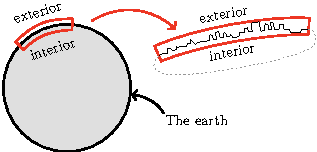
\includegraphics[width=0.6\textwidth]{figs/object_earth.pdf}
	\caption{The interior and exterior of a DTM.}
	\label{fig:object_earth}
	\end{center}
\end{figure}
Following this convention, we can still define the interior and exterior MAT of a DTM, see for instance Figure~\ref{fig:matterrain}.

A second peculiarity for DTMs is that both its interior and its exterior MAT can consist of multiple disjoint parts (also visible in Figure~\ref{fig:matterrain}), whereas for closed objects, the interior MAT always consists of one connected part. 
This is again a side effect of the open boundary.
These disjoint parts are called \emph{medial clusters}.
In most cases, one object on the terrain corresponds to one medial cluster.

% \begin{figure}
% 	\centering
% 	\begin{subfigure}{0.45\linewidth}
% 		\centering
% 		\includegraphics[width=\textwidth]{figs/watercourse_crossec_mat.pdf}
% 		\subcaption{Cross section of a watercourse. The 3D skeleton is obtained by reconstructing medial balls that touch the ground surface in two points.}\label{fig:crosssec}
% 	\end{subfigure}
% 	\qquad
% 	\begin{subfigure}{0.45\linewidth}
% 		\centering
% 		\includegraphics[width=\textwidth]{figs/watercourse_3d_mat.pdf}
% 		\subcaption{Perspective view of the 3D skeleton of simple watercourses.}\label{fig:crosssec3d}
% 	\end{subfigure}
% 	\caption[MAT segmentation]{Profile view of 3D skeleton of the terrain}
% 	\label{fig:MAT2D3D}
% \end{figure}

\section{Computing the MAT} 
Computing the MAT from the boundary $\mathcal{B}$ of an object is typically done in two steps. 
During the first step, \ie\ \emph{MAT approximation}, a noisy approximation of the MAT is obtained, and during the second step, \ie\ \emph{pruning}, the noise is removed.

\subsection{MAT approximation}
For DTMs the MAT is typically appoximated using the Voronoi diagram in case the 2D MAT is needed, or using the shrinking-ball algorithm in case the 3D MAT is needed.

% \subsubsection{Grid methods}
% Grid methods are based on the grassfire definition of the MAT and start with a binary grid that contains a rasterisation of the object boundary of interest. 
% Boundary pixels (or voxels in a 3D grid) are marked with a `0' and non-boundary pixels have the value `1'.
% From the boundary pixels the \emph{distance transform} is computed. 
% This is an image where each pixel is labeled with the distance to the nearest boundary point of the object. 
% This distance field is continuous everywhere, except at the MAT atoms where---in accordance with the grassfire analogy---the distance to the boundary decreases in at least two directions.
% These discontinuities can be detected by taking the derivative of the distance transform.

% Voxel based methods are often rotation invariant, \ie they suffer from spurious branches in the MAT when the object is not axis-aligned \citep{Borgefors08} (Figure~\ref{fig:imaimp:a} illustrates this) and sub-optimally centred, \ie the axis is not precisely medial (with the notable exception of \citet{sud2007homotopy}).
% This is due to the non-continuous and gridded coordinates the output is not rotation invariant.

% While parallelised computation is possible both for the computation of the distance transform \citep{Cao10} and the thinning methods \citep{Saha16}, this does not mean that scalability of is feasible.
% Voxel-based methods are relatively fast for small inputs, but for inputs that have a resolution of $1000^3$ voxels or more, the algorithms become significantly slower and more memory demanding since these algorithms usually scale linearly with the number of input voxels \citep{Sobiecki13}.

\subsubsection{Methods based on the Voronoi diagram}
If you compute the Voronoi diagram (VD) of a set of points on the boundary of an object, the MAT can be found by taking a subset of the edges of that VD.
This can be seen in Figure~\ref{fig:vdmat}. 
Notice that the MAT approximation becomes more accurate if more boundary points are used to compute the VD.
\begin{figure}[tbp]
	\centering
	\begin{subfigure}{0.55\linewidth}
		\centering
		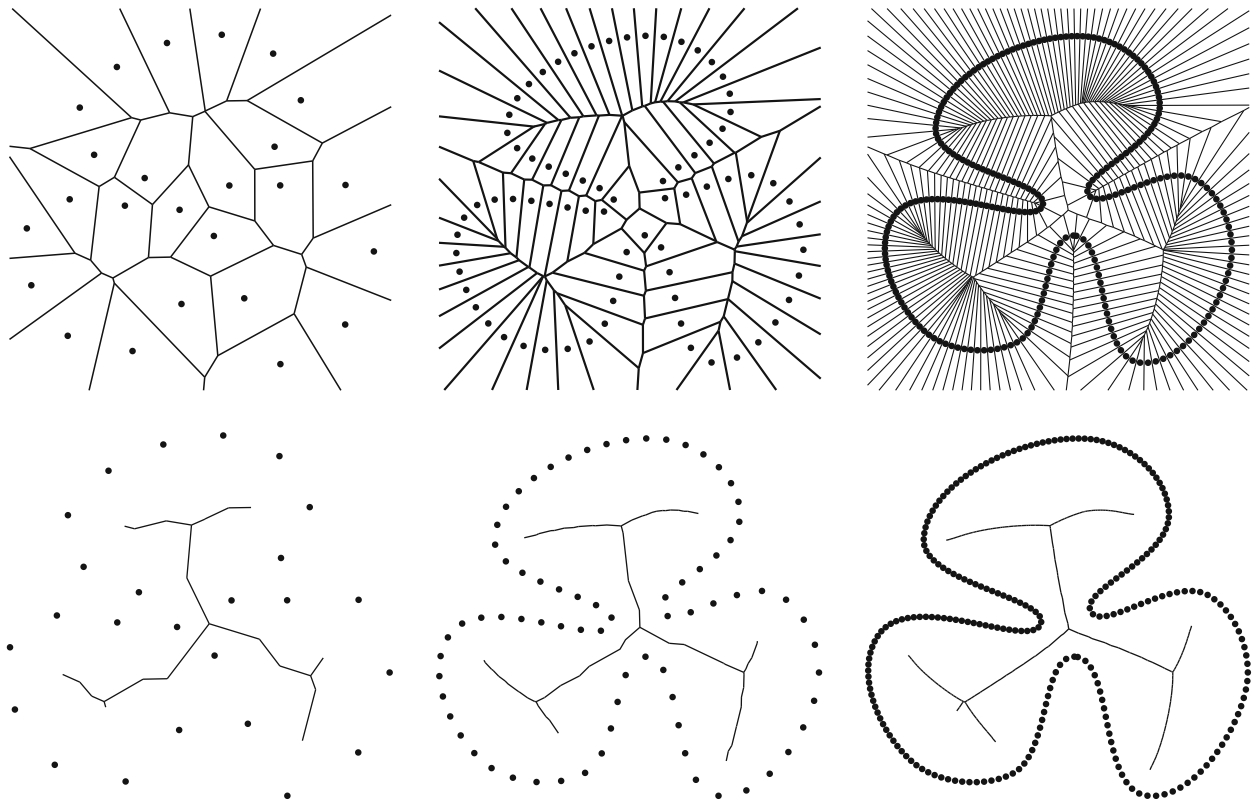
\includegraphics[width=\textwidth,angle=270]{figs/vdmat.png}
		\subcaption{Approximation of the MAT with a subset of the VD (left column). The complete VD is show in the right colomn. 
		The number of used boundary points increases from top to bottom \citep{attali1996}.}\label{fig:vdmat}
	\end{subfigure}
	\qquad
	\begin{subfigure}{0.39\linewidth}
		\centering
		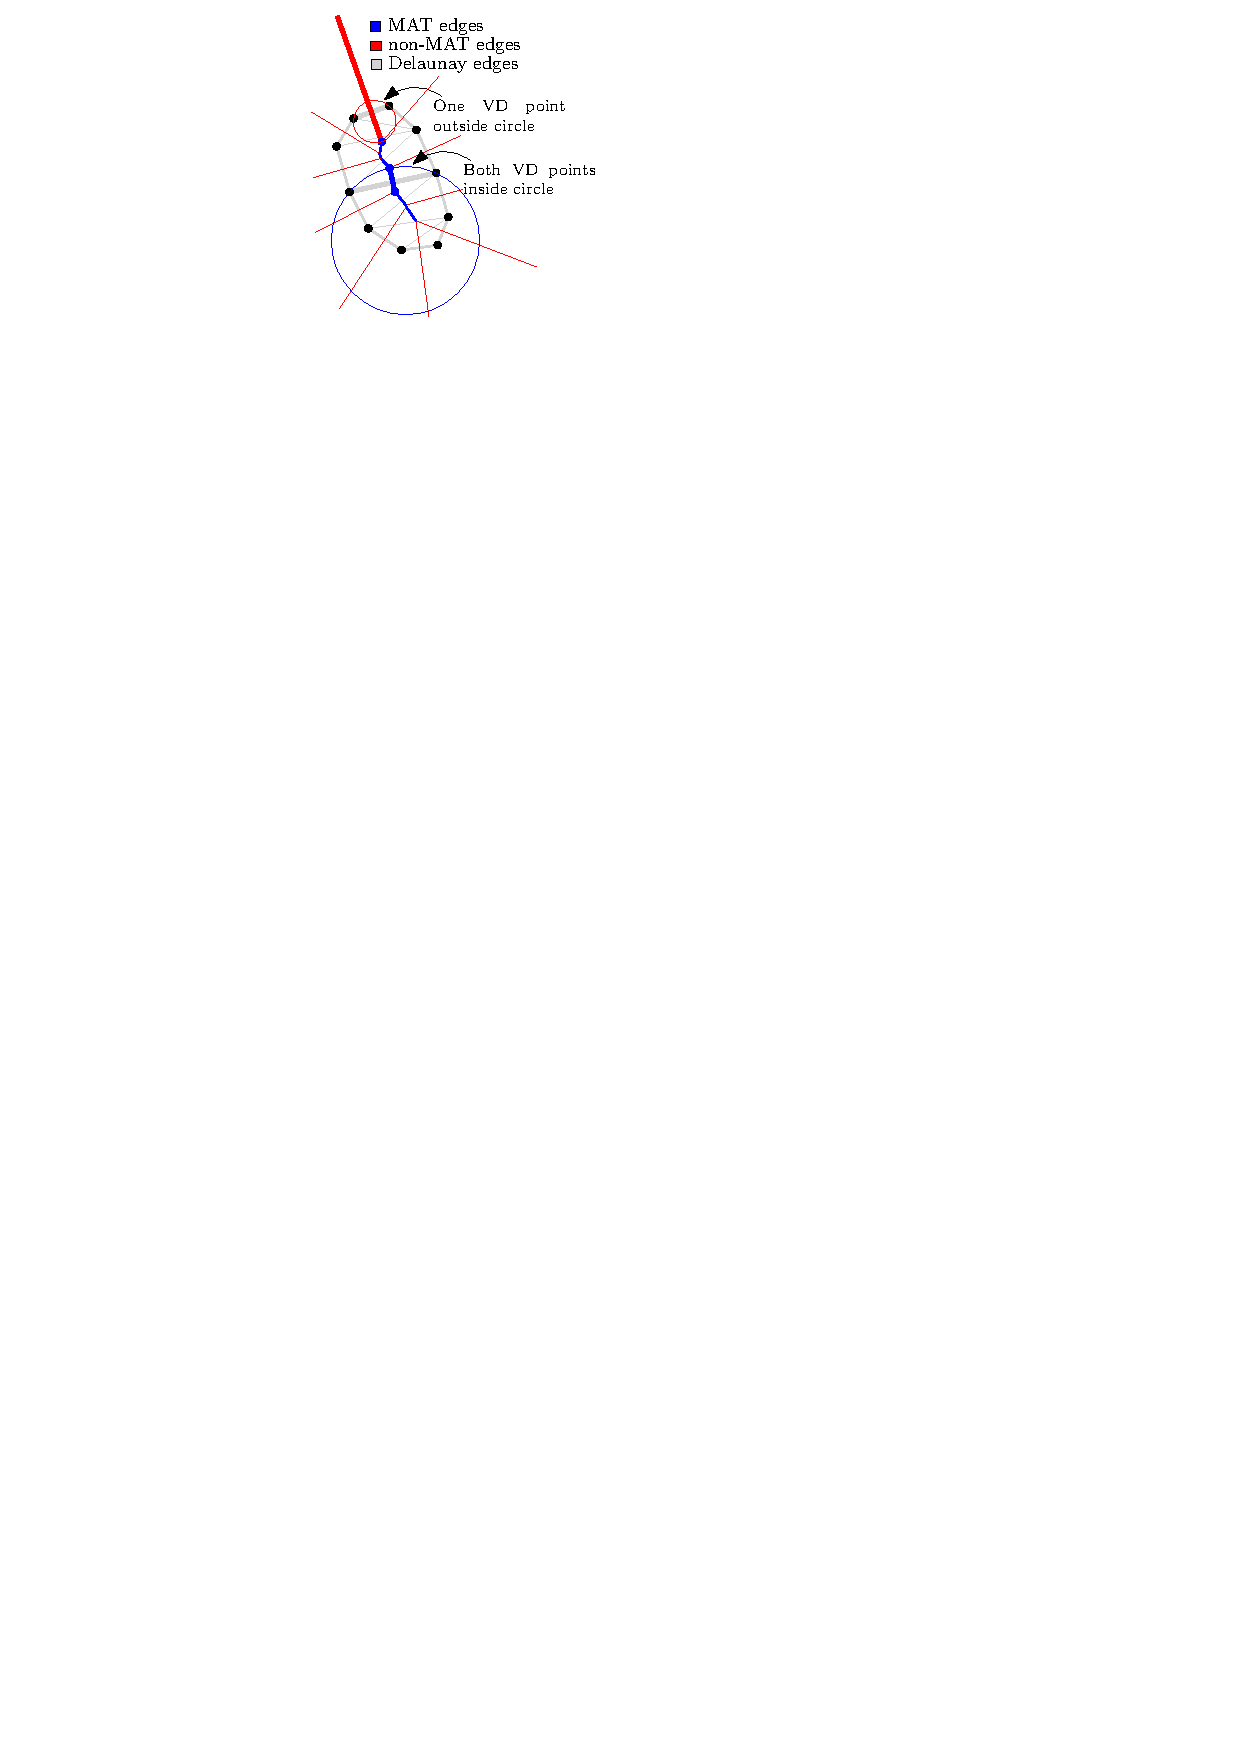
\includegraphics[width=\textwidth]{figs/one-step-crust.pdf}
		\subcaption{Selecting MAT edges from the VD by checking the `duality circles'. Boundary points drawn in black.}\label{fig:onestep}
	\end{subfigure}
	\caption{MAT approximation with the Voronoi Diagram}
	\label{fig:voronoi-mat}
\end{figure}
Voronoi-based methods revolve around selecting the correct edges from the VD that approximate the MAT.

A simple way to check if a Voronoi edge is part of the MAT is based on so-called `duality circles'.
A duality circle is defined for each pair of dual edges, \ie\ one edge from the VD and one from the DT that are each others dual. 
The duality circle is drawn through the two endpoints of the Delaunay edge and one point of the Voronoi edge (see the two circles in Figure~\ref{fig:onestep}).
If and only if the second point of the Voronoi edge lies inside the duality circle, the Voronoi edge is part of the MAT.

% Unfortunately, these results cannot be easily extended to 3D objects, because the 3D Voronoi diagram comes with several complications.
% Different algorithms and additional heuristics are needed to compute the 3D MAT of a 3D object using the 3D Voronoi diagram.
% But this is outside of the scope of this lesson.

\subsubsection{The shrinking-ball algorithm}
The shrinking-ball algorithm works well for robustly approximating the MAT of 3D objects that are represented with boundary points, \eg\ a noisy aerial lidar point cloud of a terrain would be a good candidate.
It is a simple and fast algorithm that can be made robust to noise in the boundary points.
This means that pruning the MAT after approximation is not necessary with the shrinking-ball algorithm.
The shrinking-ball algorithm takes an oriented point cloud as input, \ie\ a point cloud that includes a normal vector for each point. 
It outputs a disjoint set of medial atoms. 

The algorithm is based on the observation that the medial atom corresponding to a boundary point $\mathbf{p}$ must be positioned somewhere on the line $L$ through the normal $\vec{\mathbf{n}}$ of $\mathbf{p}$.
This observation is used to restrict the search space for the medial ball of $\mathbf{p}$ to the line $L$.
As illustrated by Figure~\ref{fig:shrinkballAlgo}, the algorithm begins with a very large candidate ball for $\mathbf{p}$ that is centered on $L$.
\begin{figure}[tbp]
	\begin{subfigure}{0.245\linewidth}
		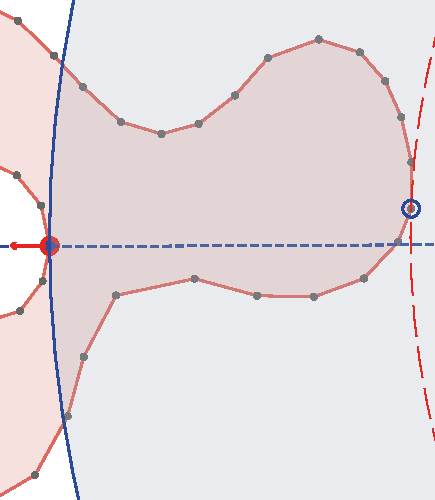
\includegraphics[width=\textwidth]{figs/fullBallShrink_1.pdf}
		\subcaption{Initial ball}
		\label{fig:fullBallShrink_1}
	\end{subfigure}
	\begin{subfigure}{0.245\linewidth}
		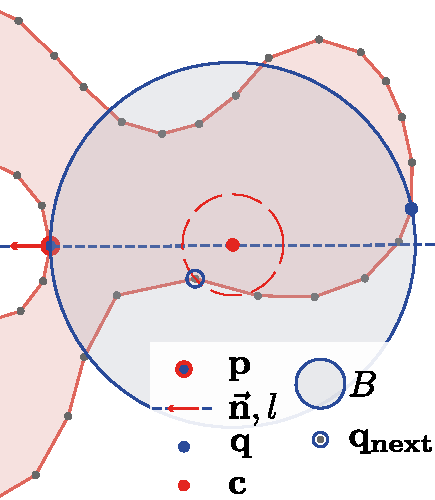
\includegraphics[width=\textwidth]{figs/fullBallShrink_2.pdf}
		\subcaption{Second iteration.}
		\label{fig:fullBallShrink_2}
	\end{subfigure}
	\begin{subfigure}{0.245\linewidth}
		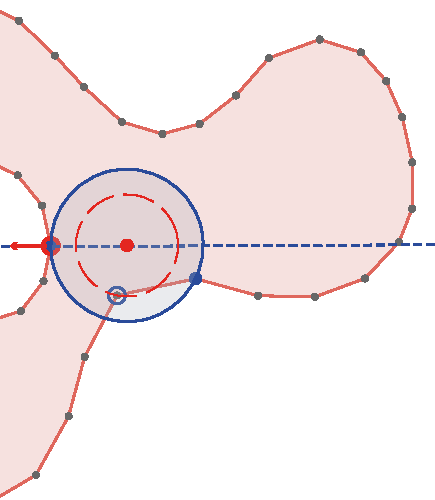
\includegraphics[width=\textwidth]{figs/fullBallShrink_3.pdf}
		\subcaption{Third iteration.}
		\label{fig:fullBallShrink_3}
	\end{subfigure}
	\begin{subfigure}{0.245\linewidth}
		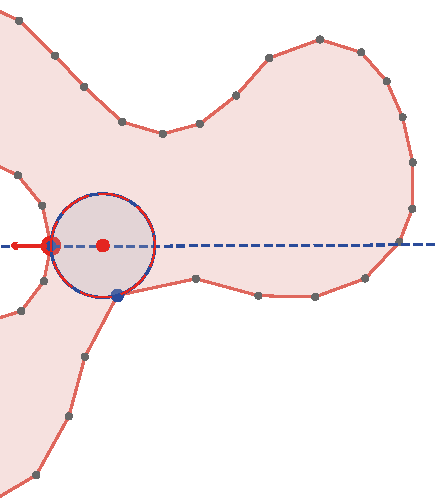
\includegraphics[width=\textwidth]{figs/fullBallShrink_4.pdf}
		\subcaption{Fourth iteration.}
		\label{fig:fullBallShrink_4}
	\end{subfigure}
	\caption{Ball shrinking iterations with the shrinking-ball algorithm. The final iteration yields a \emph{medial} ball. A legend is given in \subref{fig:fullBallShrink_2}.}
	\label{fig:shrinkballAlgo}
\end{figure}
At each consecutive iteration, a new candidate ball is constructed that is smaller than the previous one and closer to the final \emph{medial} ball.
Every ball is constructed so that it touches $\mathbf{p}$ and is centred on $L$.
Only the candidate feature point $\mathbf{q}$ changes with each iteration.
A new $\mathbf{q}$, denoted $\mathbf{q_{next}}$, is found by selecting the closest point from the centre $\mathbf{c}$ of the current ball.
Using $\mathbf{p}, \vec{\mathbf{n}}, \mathbf{q_{next}}$ we can compute the centre of the next ball $\mathbf{c_{next}}$, at which point we move on to the next iteration.
The algorithm terminates when an empty ball is found, which is the case when the radius no longer shrinks.
Algorithm~\ref{alg:shrinkBall} gives the pseudo-code for the shrinking-ball algorithm.
\begin{algorithm}[tb]
	\SetKwInOut{Input}{Input}
	\SetKwInOut{Output}{Output}
	\DontPrintSemicolon\Input{
		a KD-tree of the surface point cloud $T$,\\ 
		a surface point $\mathbf{p}$\\ 
		it's normal vector $\vec{\mathbf{n}}$, and\\
		the initial ball radius $r_{init}$}
	\Output{the medial ball centre $\mathbf{c}$,\\the medial ball radius $r$}
	$r \leftarrow r_{init}$ \\
	$\mathbf{c} \leftarrow$ the centre of the ball that touches $\mathbf{p}$ is centered on $\vec{\mathbf{n}}$ with a radius $r$ \\
	\Repeat{a \textbf{break} statement is executed} {
		$q_{next} \leftarrow$ the nearest point to $\mathbf{c}$, obtained quickly using $T$ \\
		$r_{next} \leftarrow$ radius of the next ball that touches $\mathbf{p}$ and $\mathbf{q_{next}}$ and is centred on $\vec{\mathbf{n}}$ \\
		$\mathbf{c_{next}} \leftarrow$ centre of the next ball, can be computed with $\mathbf{p}, \vec{\mathbf{n}}$, and $r_{next}$ \\
		\If{$r_{next} = r$} {
			\textbf{break}
		}
		$\mathbf{c} \leftarrow \mathbf{c_{next}}$ \\
		$r \leftarrow r_{next}$
	}
	\caption{The shrinking-ball algorithm.}
	\label{alg:shrinkBall}
\end{algorithm}

The algorithm is run for each point in the input point cloud. 
If the normal vectors point away from the interior, the interior MAT is computed.
And by flipping the orientation of the normal vector, the exterior MAT can also be computed.
If normals are not available for a point cloud, these can be estimated using local plane fitting, \ie\ by fitting a plane to the $k$ nearest neighbours of each boundary point. 
The vector perpendicular to that plane then becomes the estimated normal vector.
A KD-tree is typically used to speed up the nearest neighbour searches, both for normal estimation and the shrinking-ball algorithm.
Figure~\ref{fig:ca_ridge} gives an example result of the shrinking-ball algorithm for a terrain point cloud. 
Observe how the MAT describes the valleys (exterior MAT) and ridges (interior MAT) in the terrain with its skeletal structure.
\begin{figure}
	\centering
	\begin{subfigure}{0.310\linewidth}
		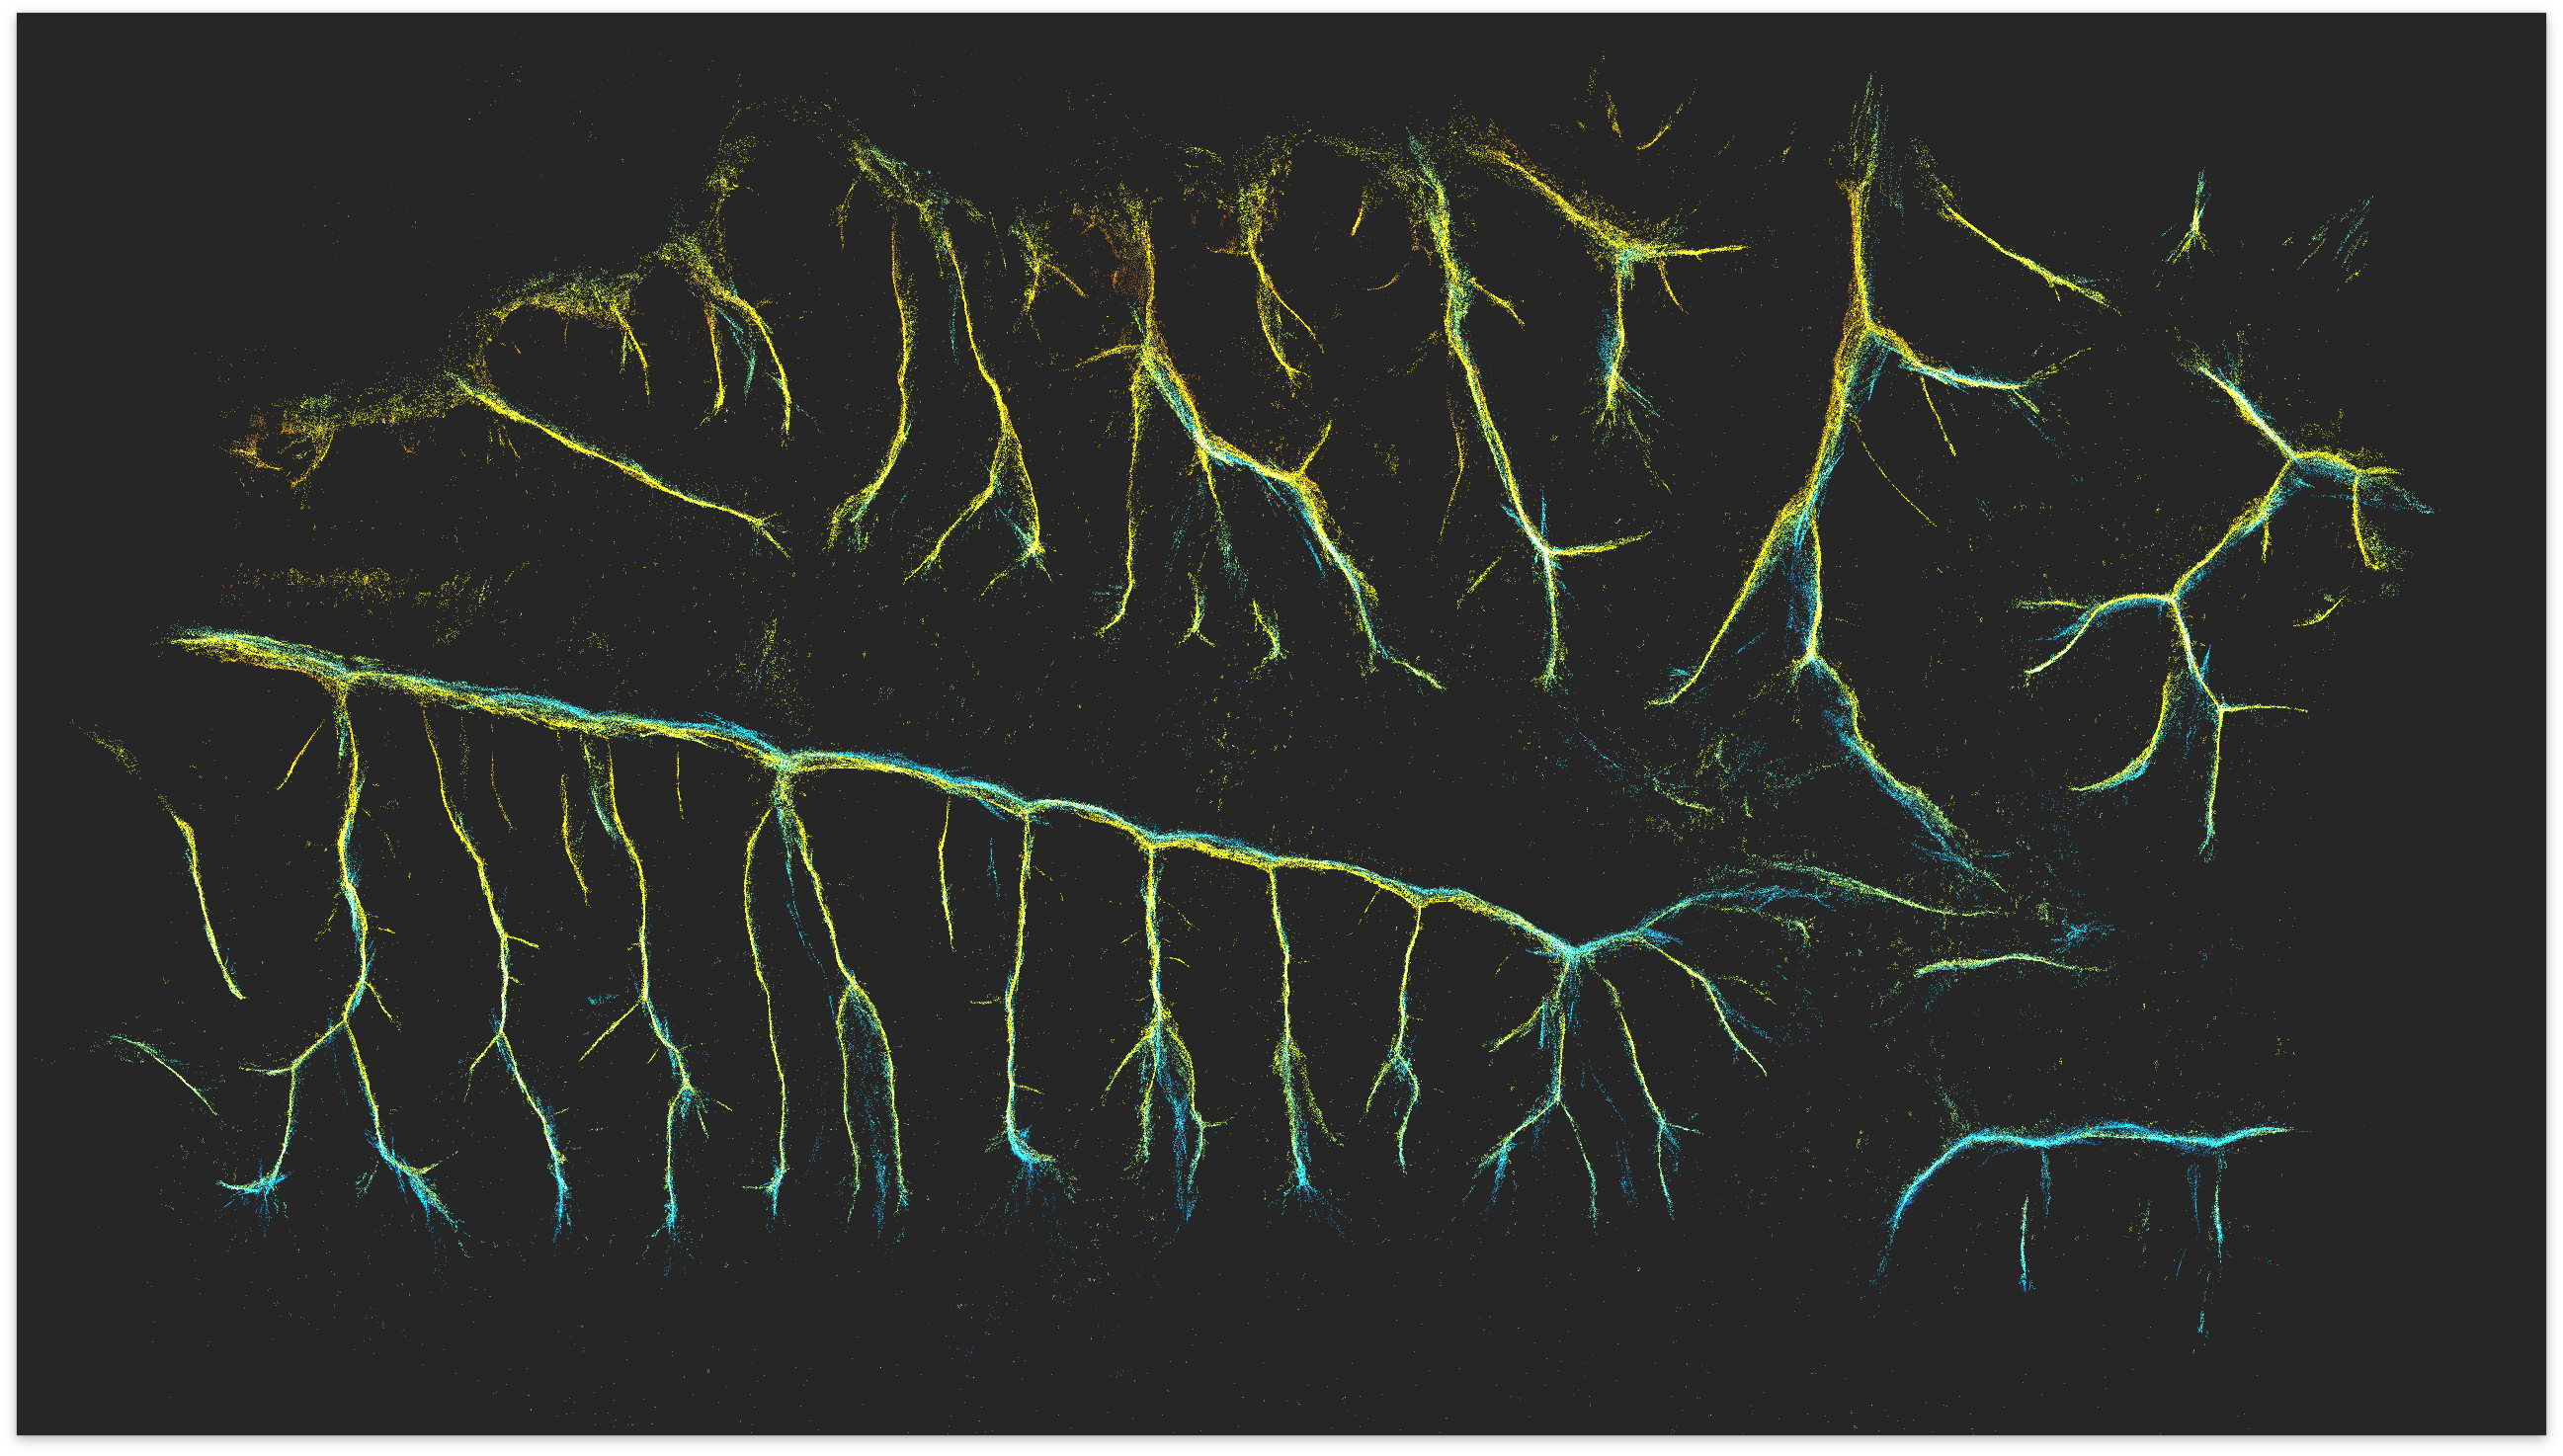
\includegraphics[angle=90,width=\linewidth]{figs/iMAT.png}
		\caption{Interior MAT.}
		\label{fig:ca_ridge:imat}
	\end{subfigure}
	\quad
	\begin{subfigure}{0.310\linewidth}
		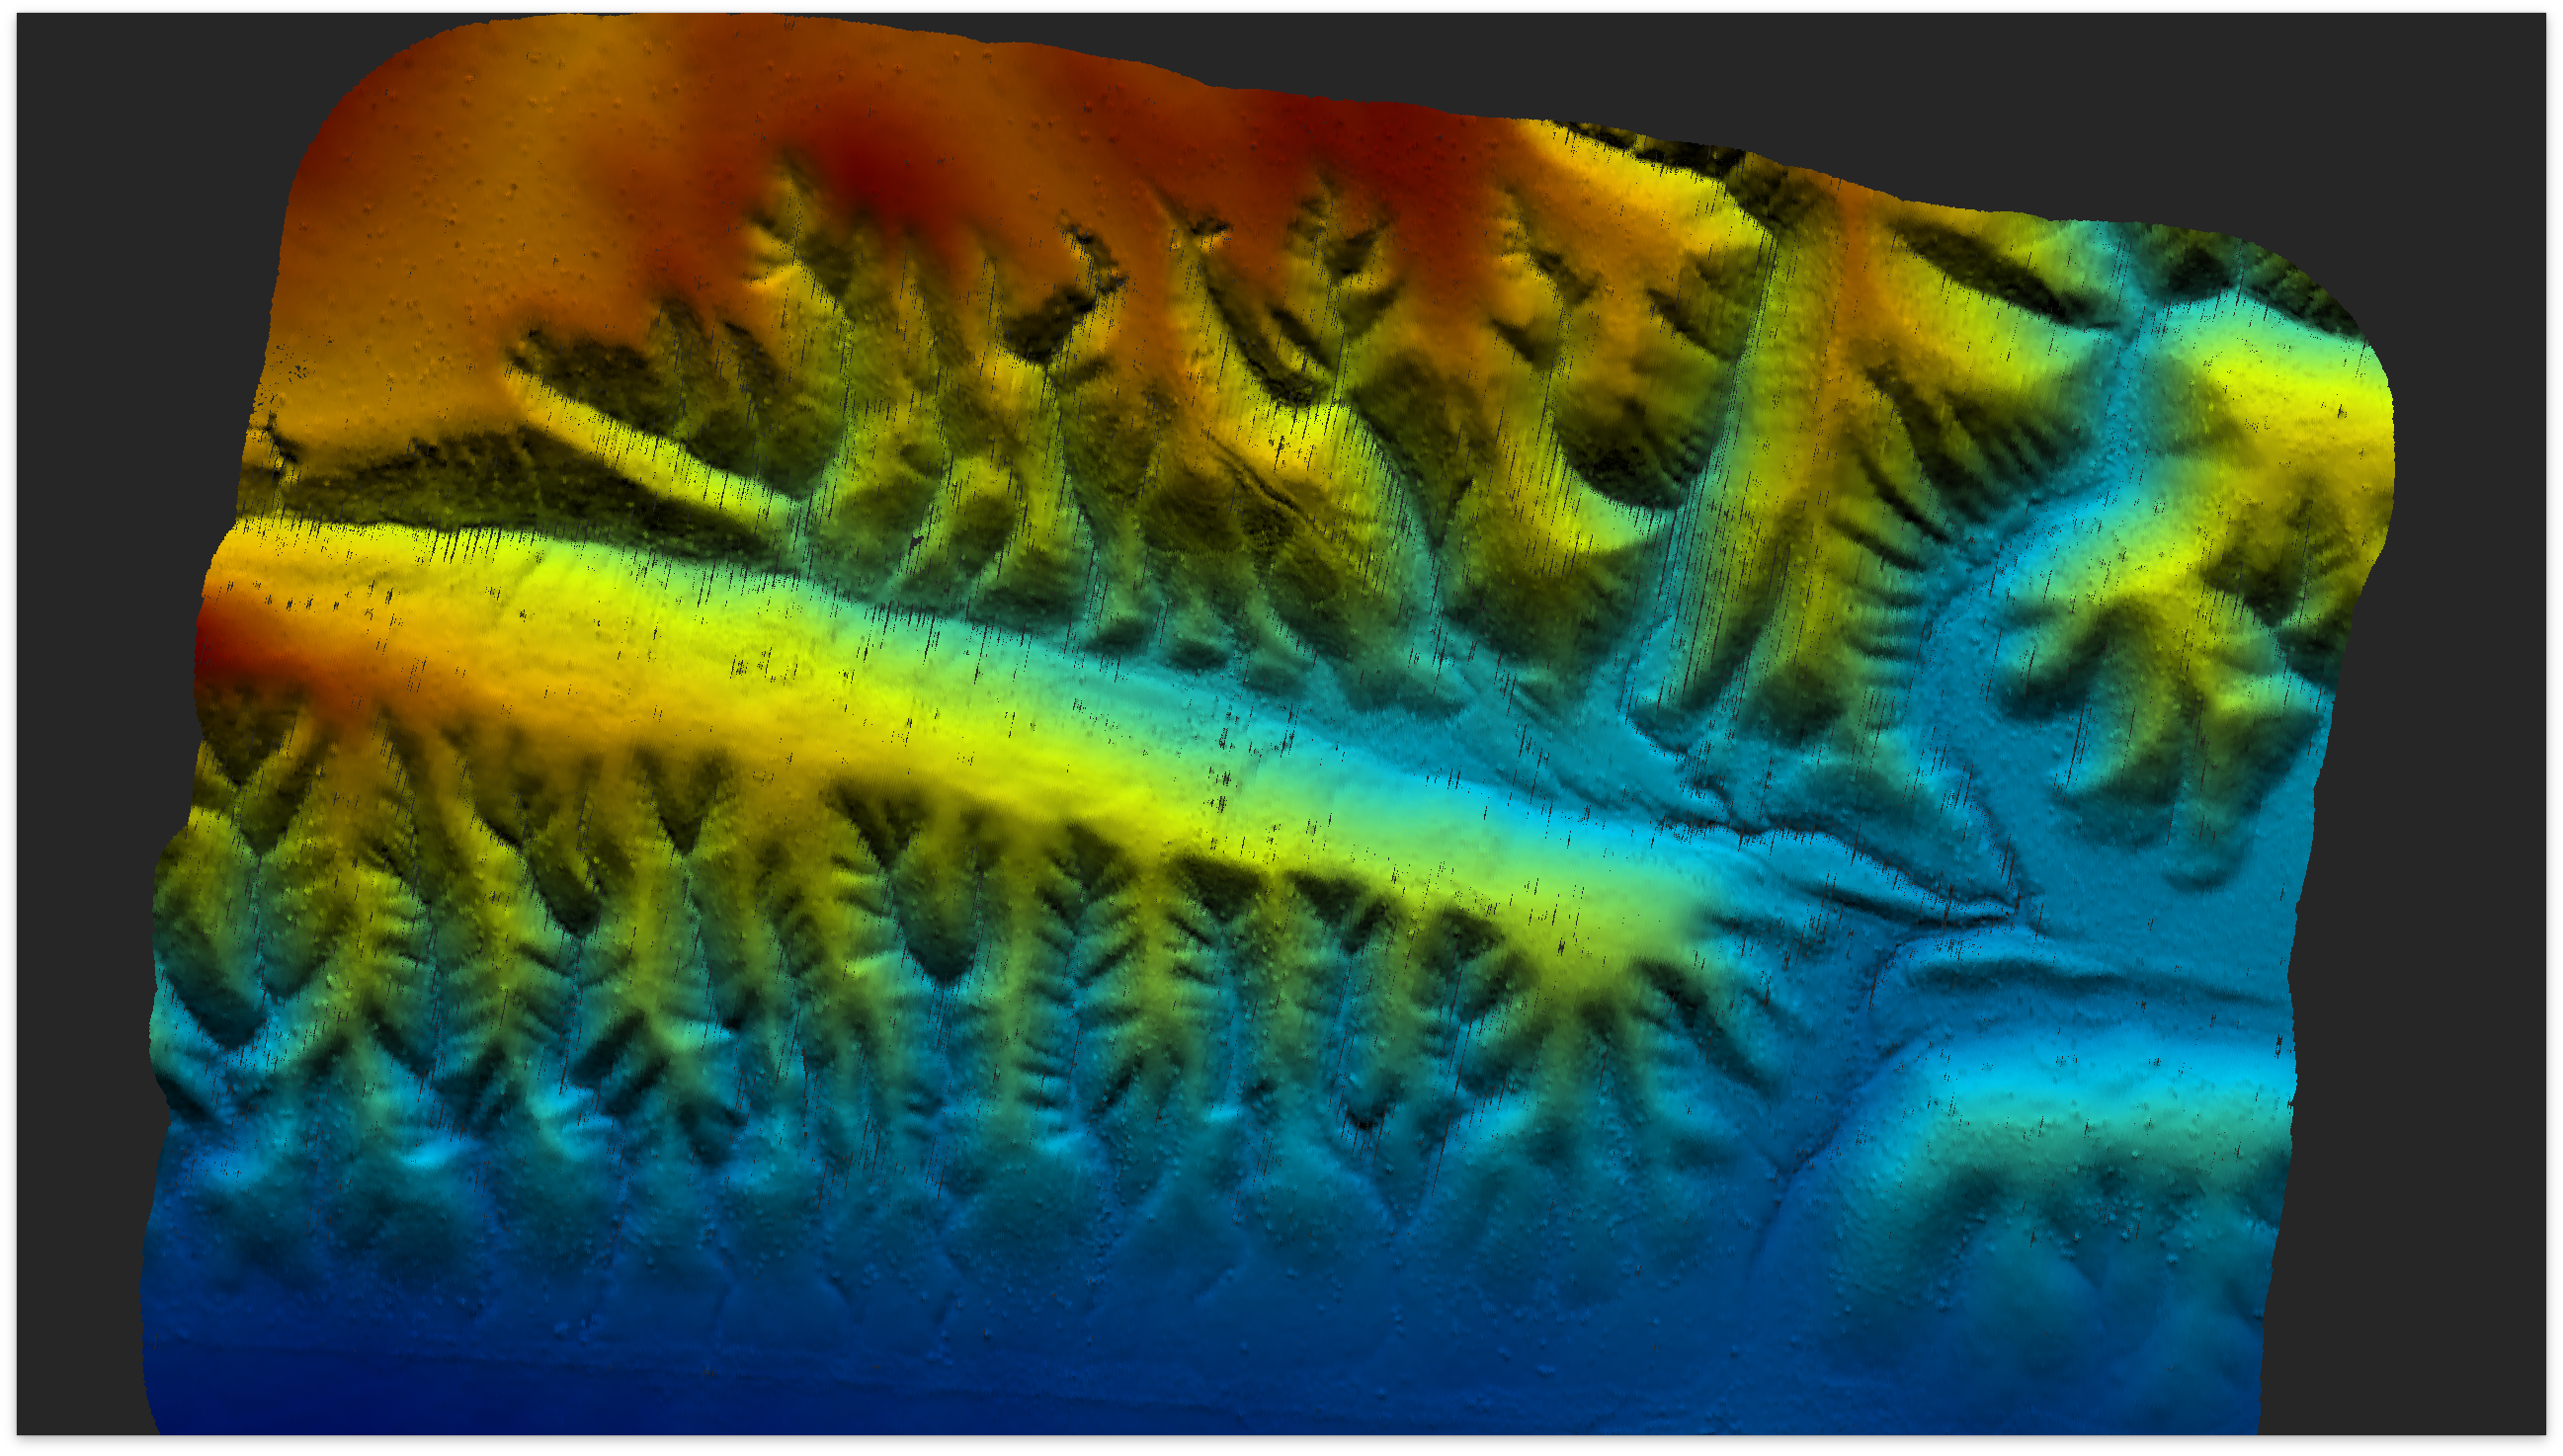
\includegraphics[angle=90,width=\linewidth]{figs/terrain.png}
		\caption{Terrain points}
		\label{fig:ca_ridge:terrain}
	\end{subfigure}
	\quad
	\begin{subfigure}{0.310\linewidth}
		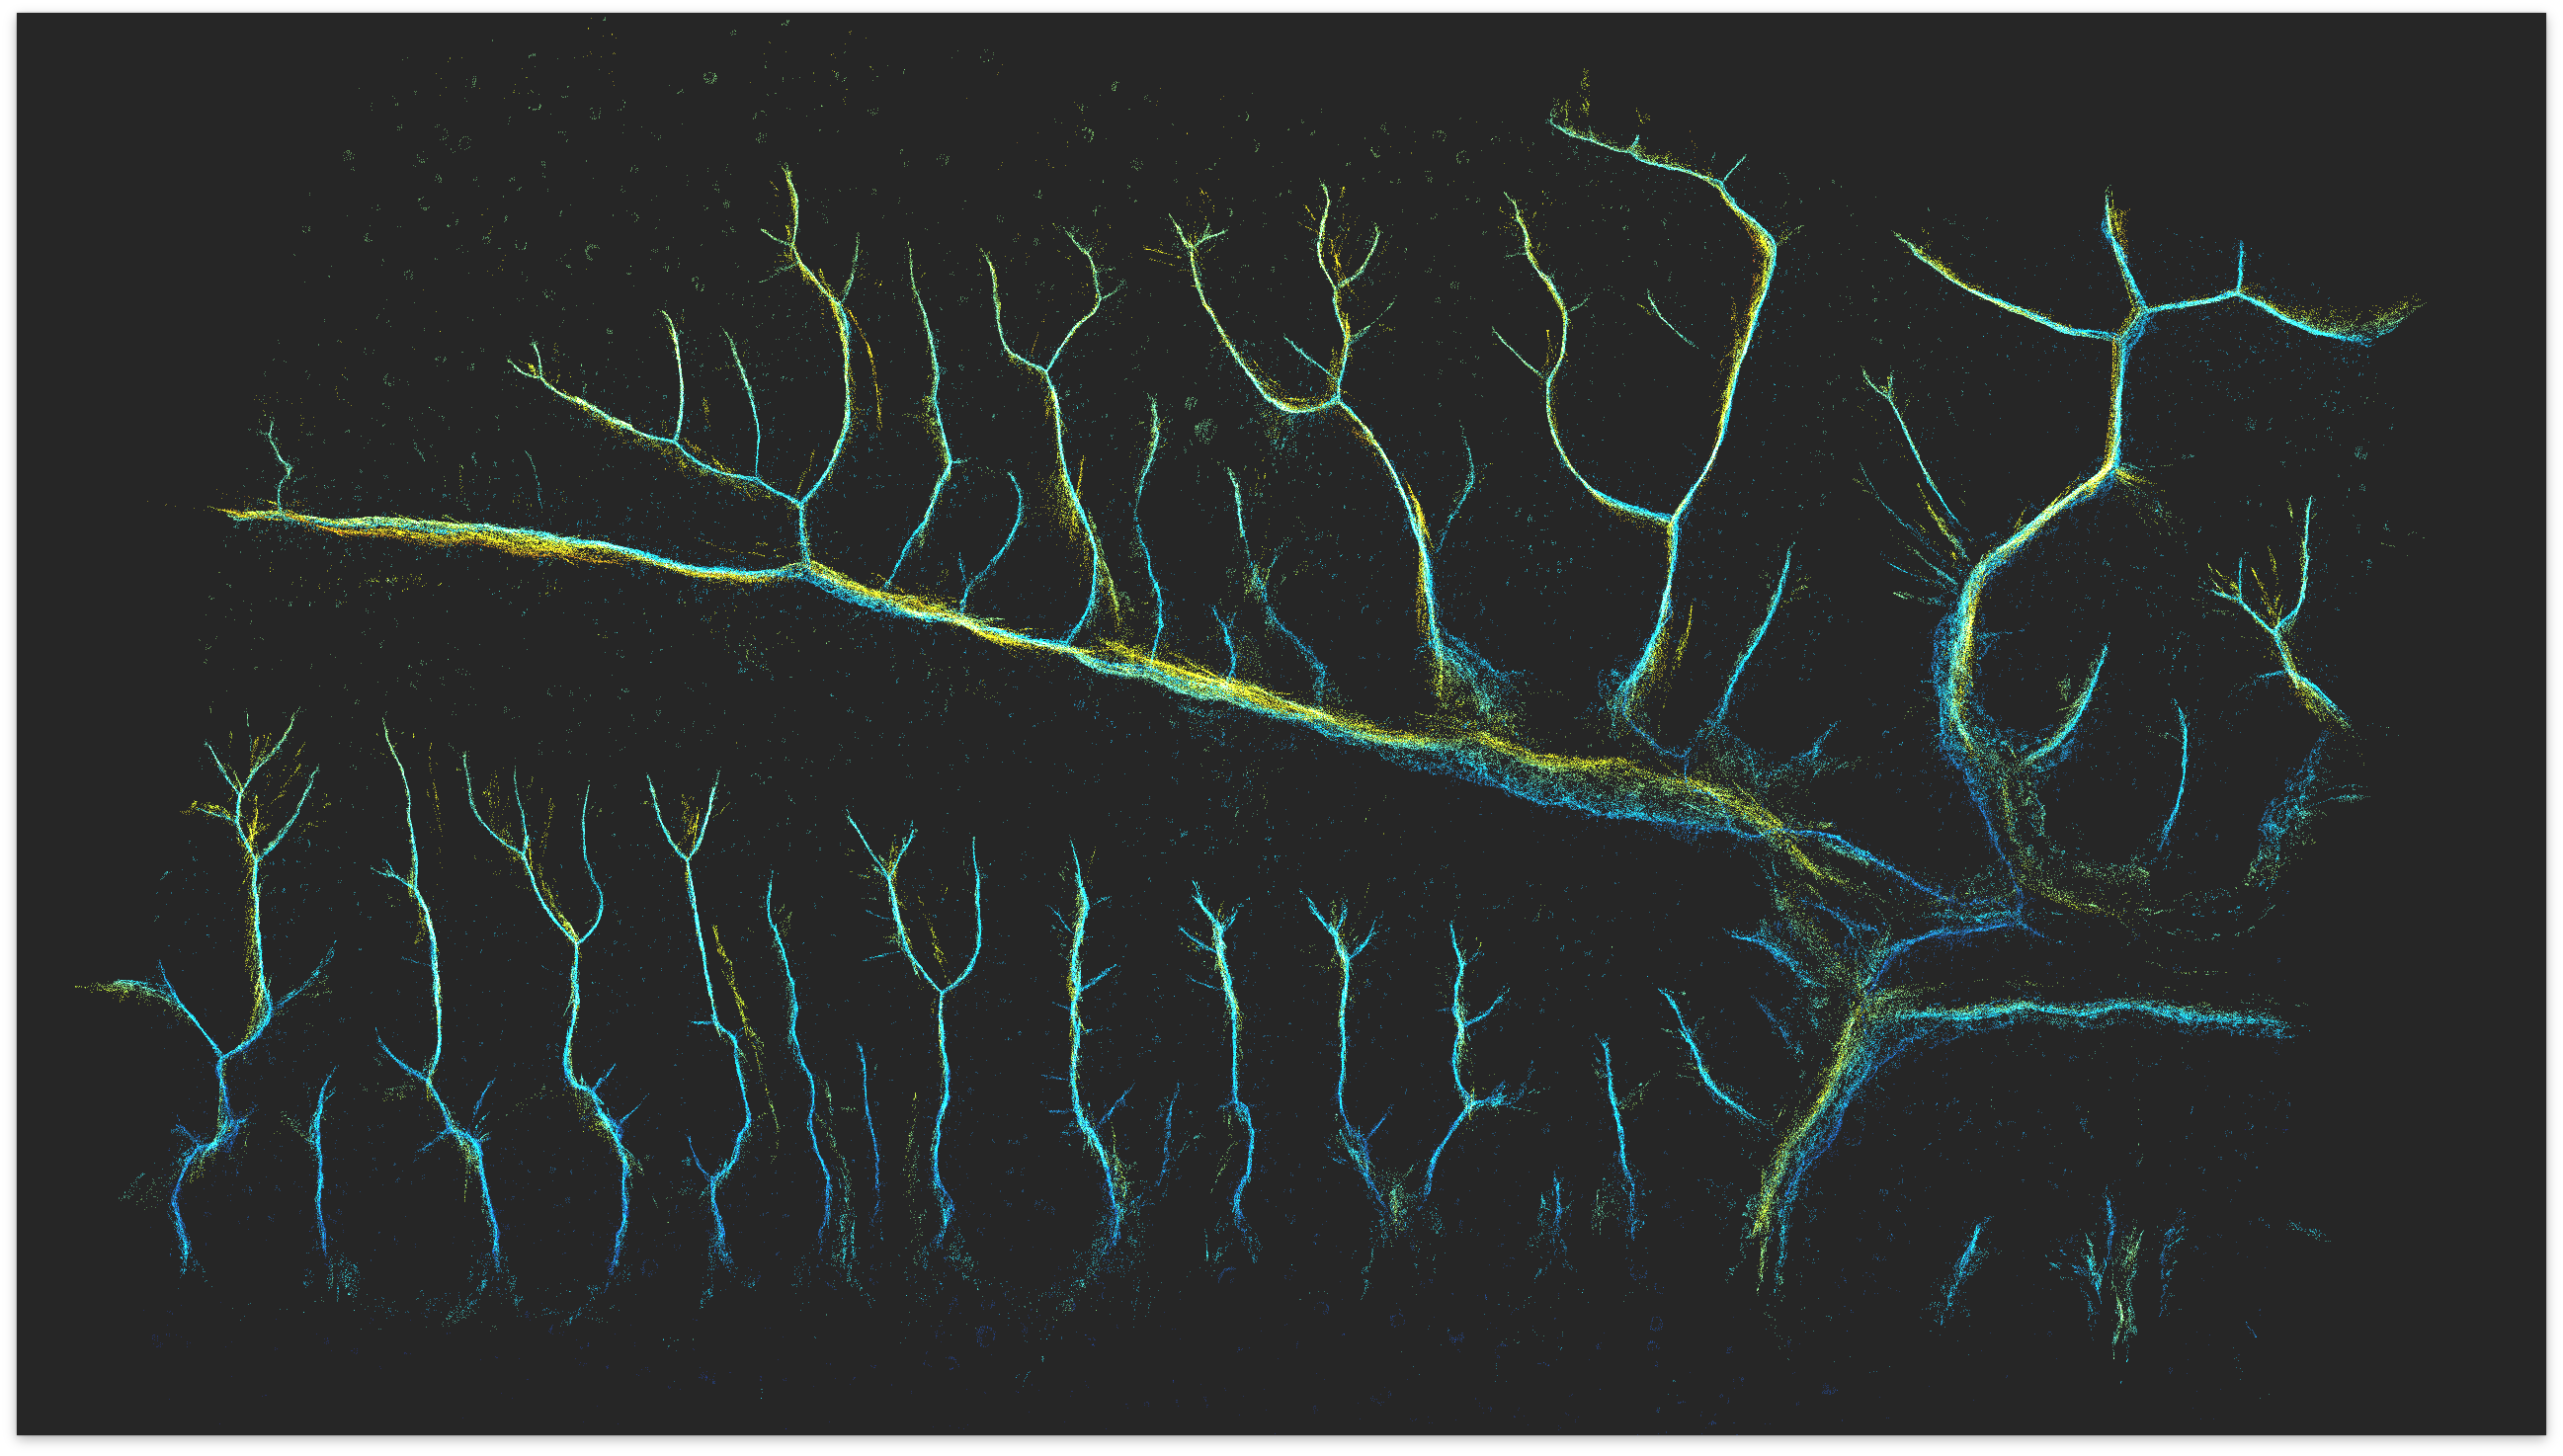
\includegraphics[angle=90,width=\linewidth]{figs/oMAT.png}
		\caption{Exterior MAT}
		\label{fig:ca_ridge:omat}
	\end{subfigure}
	\caption{MAT approximation (a,c) of a lidar terrain point cloud (b) obtained with the shrinking-ball algorithm. Top view.}
	\label{fig:ca_ridge}
\end{figure}

% The main limitation of the shrinking-ball algorithm is that it outputs only an unstructured set of medial atoms, \ie\ there is no distinction between its different medial sheets.% and also the surface of the sheets is not explicitly reconstructed.
% This can be solved by using the medial geometry of the medial atoms.
% Several properties of the medial geometry are locally similar within the same medial sheet.
% With a region-growing algorithm this similarity can be exploited to segment the unstructured medial atoms into medial sheets.
% Especially the medial bisector is useful, \ie\ it is tangential to the medial sheet and it always points in the direction of decreasing radius in a sheet, usually away from junction curves.
% It is thus not only similar within one sheet, but also dissimilar for the different sheets that meet at a junction curve.
% As a result there is little chance that a sheet segment grows into another sheet through a junction curve, leading to well separated sheets (see Figure~\ref{fig:MATmeth}).
% Region-growing can also be used to segment the MAT of a DTM in its different disjoint medial clusters.
% In this case the region-growing condition may be based on a measure for the amount of overlap between nearby medial balls.
% Because, nearby medial balls within one medial cluster are likely to overlap, whereas medial balls between different clusters are not.

%% Structuration is the process of overcoming this limitation by constructing the sheet surfaces, \eg as a triangular mesh, from which explicit structural information about the hierarchy of the MAT can be obtained \citep{Delame16}.

\subsection{Pruning}
Pruning is the process of retracting or removing unimportant branches from the MAT.
It is often necessary because the MAT is unstable, \ie\ it is extremely sensitive to small bumps in $\mathcal{B}$.
As illustrated in Figures~\ref{fig:mat-instability} and \ref{fig:imaimp:a}, tiny deviations in $\mathcal{B}$ can lead to big spurious branches in the structure of the MAT.
\begin{figure}
	\centering
	\begin{subfigure}{0.425\linewidth}
		\centering
		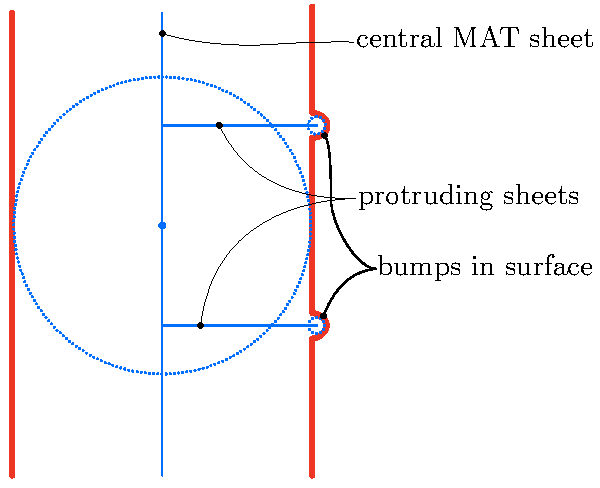
\includegraphics[width=\textwidth]{figs/protrudingSheets.pdf}
		\subcaption{Small bumps in the boundary can cause big spurious branches to appear. Object boundary drawn in red, MAT in blue.}\label{fig:mat-bumps}
	\end{subfigure}
	\qquad
	\begin{subfigure}{0.50\linewidth}
		\centering
		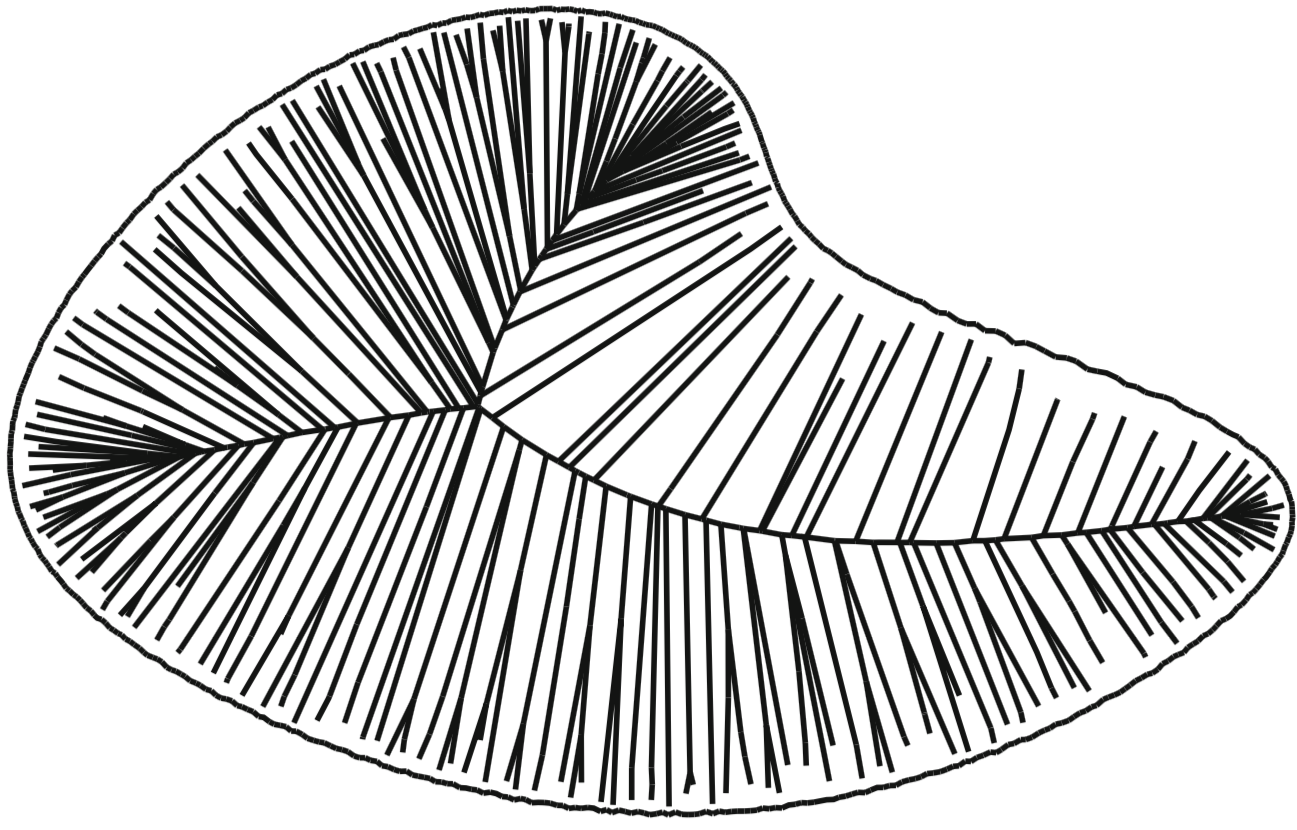
\includegraphics[width=\textwidth]{figs/spurious_branches.png}
		\subcaption{Spurious branches can appear in the MAT due to a small amount of noise in the boundary.}
		\label{fig:sb_noise}
	\end{subfigure}
	\caption{Instability of the MAT.}
	\label{fig:mat-instability}
\end{figure}
This is especially problematic when $\mathcal{B}$ has some noise as is the case with the typical DTM.
The resulting MAT can become so distorted by the spurious branches that it becomes hard to distinguish its main medial structure.
The main aim of pruning is to remove these spurious branches.

Most pruning methods are based on the properties of the medial geometry. 
Based on these properties, an importance measure for each medial atom is defined, which is then used as a threshold to filter medial atoms. 
The resulting (pruned) MAT is usually a subset of the original MAT. 
Some methods preserve topology, others do not or do so only up to a certain level. 
The main challenge is often selecting the optimal threshold value---a compromise between removing noisy MAT parts and not removing fine detail, \ie often the endpoints of good MAT branches are also affected by pruning.
Examples of importance measures for pruning are the separation angle $\theta$ (recall this is the angle between the spoke vectors) and the separation distance $\lambda$, \ie the distance between the two feature points of a medial atom. 
These values are typically low for noisy parts of the MAT.
Figure~\ref{fig:imaimp} gives an example of pruning with the separation distance.
\begin{figure}
	\centering
	\begin{subfigure}{0.4\linewidth}
	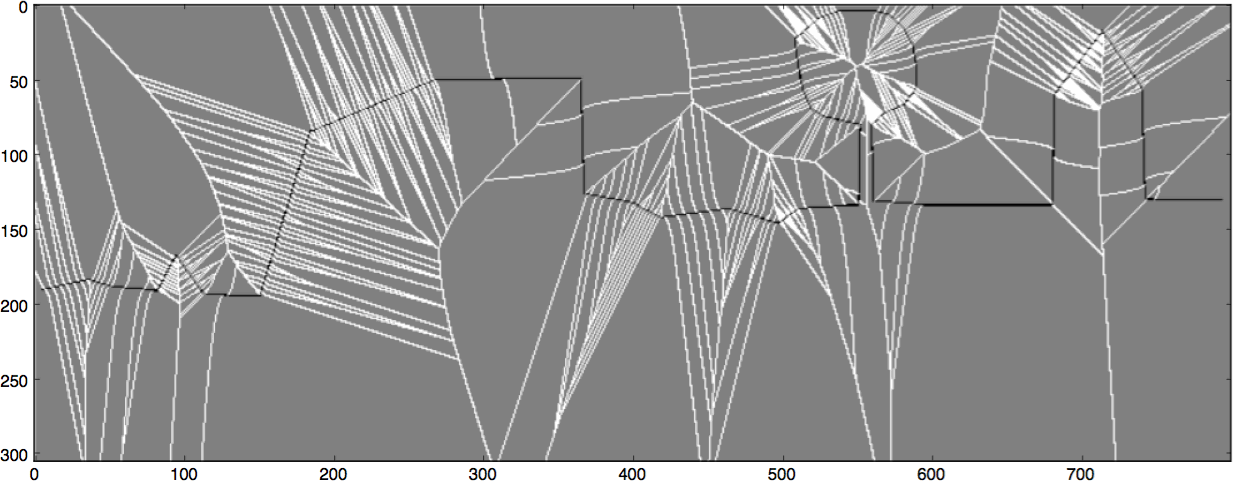
\includegraphics[width=\linewidth]{figs/rasterimpl/simple_dtm-gamma1_earthskel_.png}
	\caption{MAT without pruning ($\lambda=0$)}
	\label{fig:imaimp:a}
	\end{subfigure}
	\quad
	\begin{subfigure}{0.4\linewidth}
	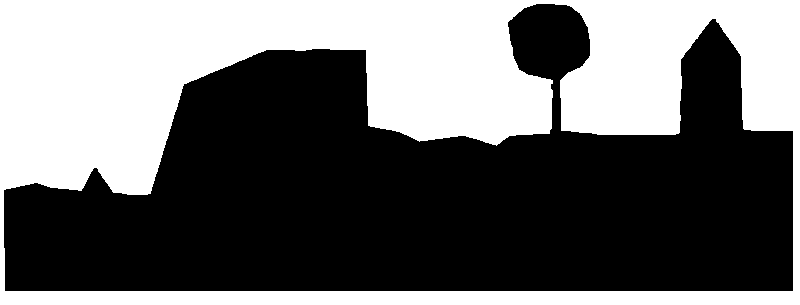
\includegraphics[width=\linewidth]{figs/rasterimpl/simple_dtm-gamma1_earthskel.png}
	\caption{Reconstructed object for $\lambda=0$.}
	\label{fig:imaimp:b}
	\end{subfigure}
	
	\begin{subfigure}{0.4\linewidth}
	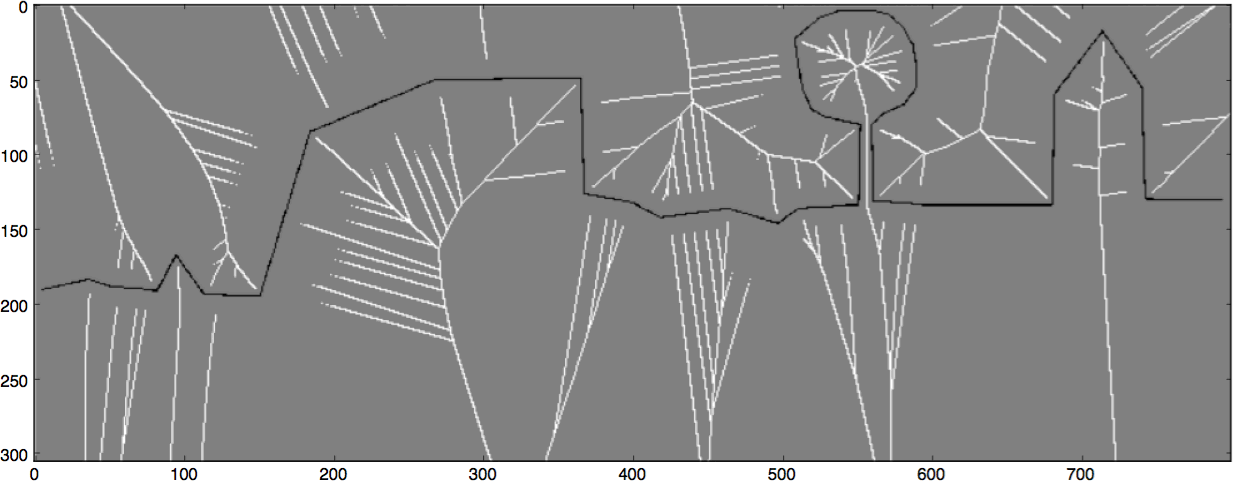
\includegraphics[width=\linewidth]{figs/rasterimpl/simple_dtm-gamma6_earthskel_.png}
	\caption{MAT with medium pruning ($\lambda=6$)}
	\label{fig:imaimp:c}
	\end{subfigure}
	\quad
	\begin{subfigure}{0.4\linewidth}
	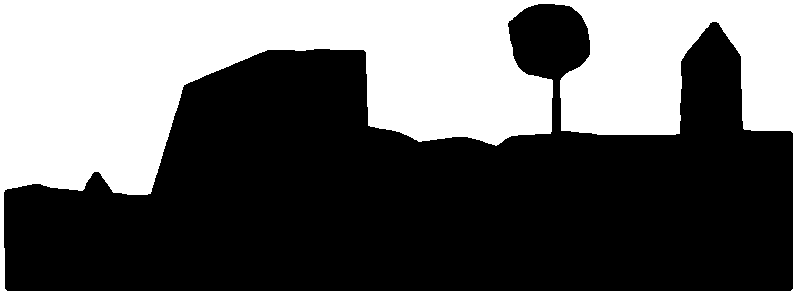
\includegraphics[width=\linewidth]{figs/rasterimpl/simple_dtm-gamma6_earthskel.png}
	\caption{Reconstructed object for $\lambda=6$. Despite the pruned MAT, the corresponding boundary remains almost unchanged.}
	\label{fig:imaimp:d}
	\end{subfigure}
	
	\begin{subfigure}{0.4\linewidth}
	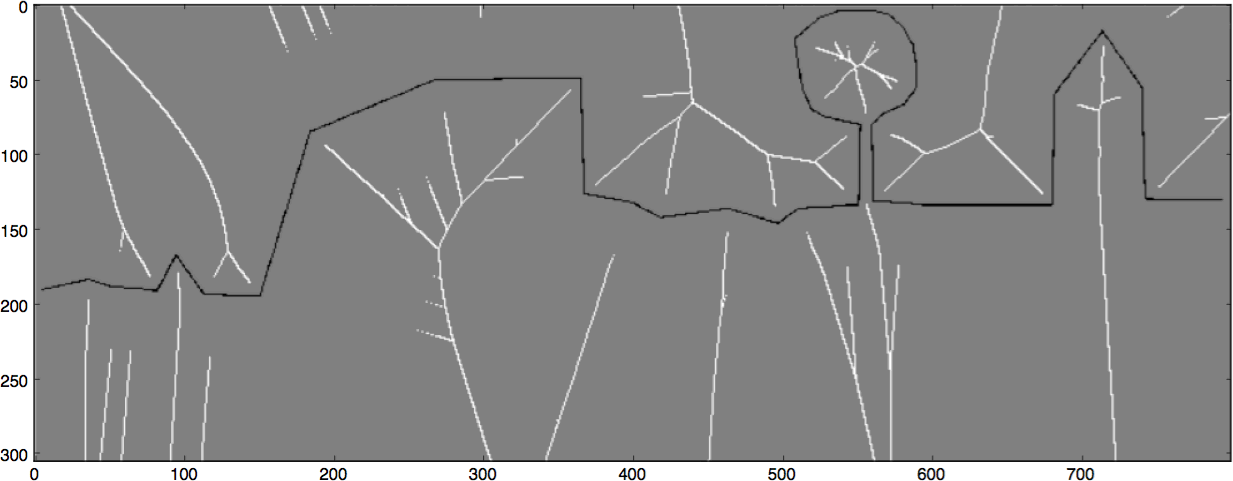
\includegraphics[width=\linewidth]{figs/rasterimpl/simple_dtm-gamma10_earthskel_.png}
	\caption{MAT with strong pruning ($\lambda=10$).}
	\label{fig:imaimp:e}
	\end{subfigure}
	\quad
	\begin{subfigure}{0.4\linewidth}
	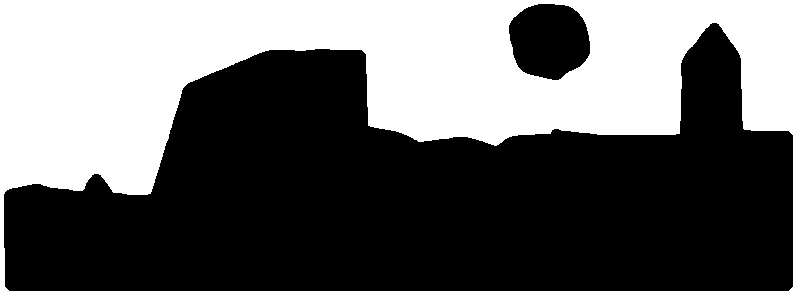
\includegraphics[width=\linewidth]{figs/rasterimpl/simple_dtm-gamma10_earthskel.png}
	\caption{Reconstructed object for $\lambda=10$. Notice how the tree is separated from the the ground and that edges have become rounder.}
	\label{fig:imaimp:f}
	\end{subfigure}
	\caption{The effect of different levels of pruning on the MAT.}
	\label{fig:imaimp}
	\end{figure}

% Pruning is virtually always performed as a post-process when the MAT is approximated using a grid method or a method based on the Voronoi Diagram, extremely clean inputs excepted.
% The shrinking ball algorithm, on the other hand, can be modified in such a way that its output does not require pruning afterwards.
% The modification boils down to checking during each iteraions the separation angle of the candidate medial ball.
% When the separation angle drops below a threshold, the algorithm is terminated and the current candidate ball is picked as the definitive medial ball for the current boundary point.
% This is illustrated in Figure~\ref{fig:sb_noise}, \ie\ because the separation angle $\theta_{i+1}$ of the next atom is very small, the shrinking ball process is terminated at the current atom $\mathbf{c_i}$.
% Notice that the separation angle became so small because the candidate feature point `jumped' from one side of the boundary to the other side (compare $\mathbf{q_i}$ and $\mathbf{q_{i+1}}$).
% This typically happens in the presence of noisy boundary points, and illustrates why filtering on a low separation angle is effective for pruning.

\section{Applications of the MAT for DTMs}
% Following is a list with applications of both the 2D and the 3D MAT for DTMs. 
There are several applications of the 2D MAT.
Often it is applied on sets of lines such as isolines or river networks to perform operations that require the preservation of topology, \ie\ there should not be any self-intersections or intersection between neighbouring lines.
This is often a problem with methods that treat the lines separately without considering the complete system of lines.
However, by working on the MAT, and keeping the boundary in sync during the MAT processing, this requirement can be satisfied rather easily.

For example, \citet{Gold01b} generalise the isolines, \ie\ to simplify their appearance for (small scale) map production. 
This is achieved by pruning spurious branches from the MAT and then reconstructing the isolines from the pruned MAT. 
The method also works for river networks.

\citet{Karimipour13} describe a way to estimate catchment areas based solely on the MAT of an existing river network.
A catchment area is a hydrological unit where precipitations that fall into this area, eventually end up in the same river. 
Ideally, these areas are computed based on the elevation of a DEM by simulating the natural flow of water. 
However, this can be a very time consuming process and the elevation data may not always be available, and with the MAT, a quick and reasonable approximation of catchment areas can be obtained.
The catchment areas are polygons that are constructed by connecting several simplified MAT branches.

Finally, \citet{Dakowicz03} demonstrate how the MAT can be used to solve the wedding cake effect for TINs that was described in Lesson 08. 
Recall that this effect happens because sometimes flat triangles are created between the vertices of one isoline.
The problem is solved by adding points with a plausible elevation along the MAT between the isolines prior to triangulation.

The idea of applying the 3D MAT to digital terrain modelling is still relatively new.
As mentioned in the introduction of this lesson, one interesting application is object detection in a terrain.
\citet{Broersen17} show how the 3D MAT, computed with the shrinking-ball algorithm, can be used to detect watercourses in the Dutch landscape (see Figure~\ref{fig:MATsegmentation}). 
\begin{figure}
	\centering
	\begin{subfigure}{0.5\linewidth}
		\centering
		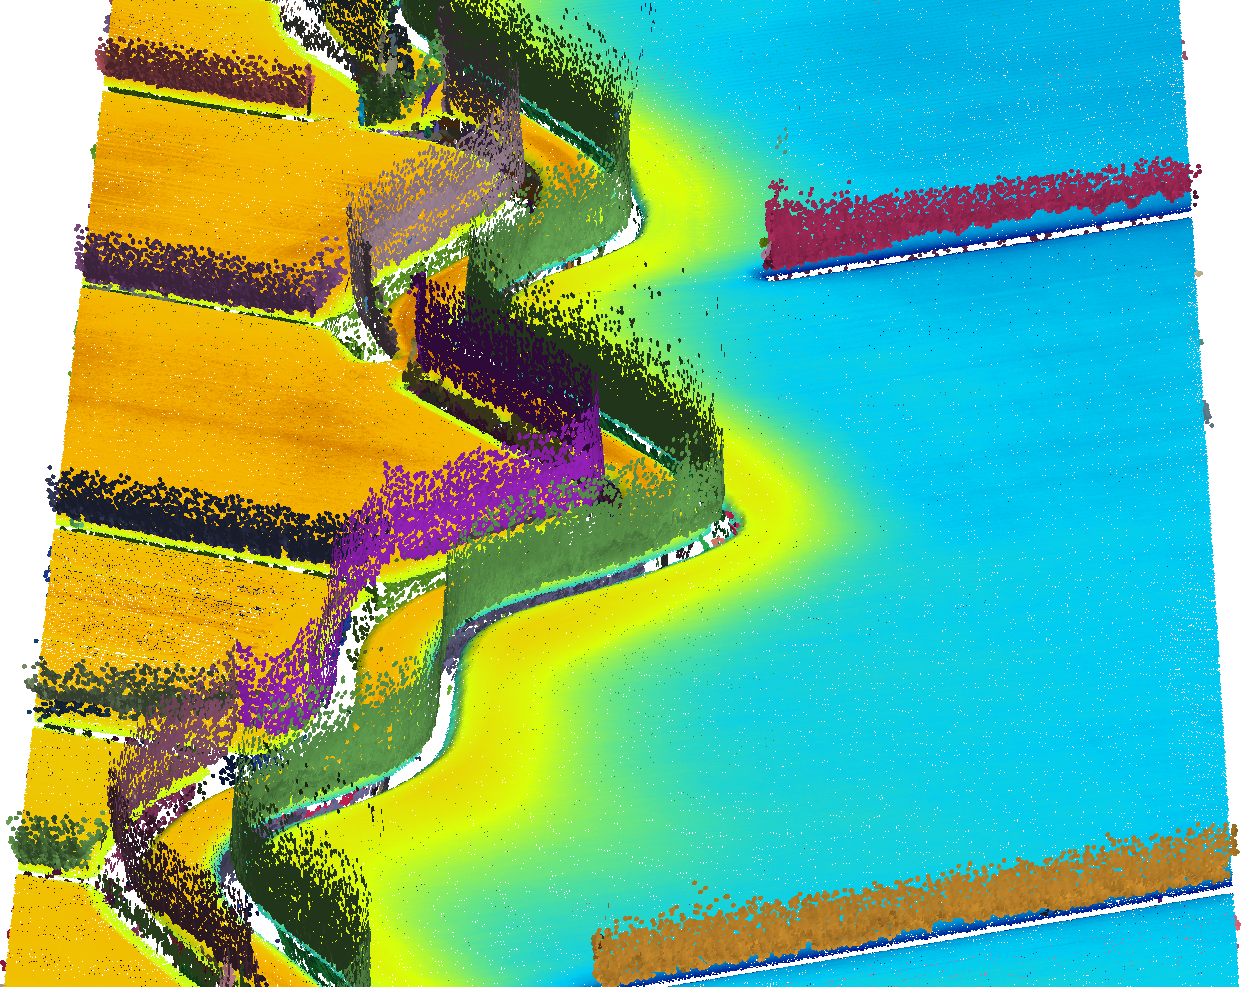
\includegraphics[width=\textwidth]{figs/3dmat.png}
		\subcaption{Perspective view of exterior MAT and ground points of a terrain with several watercourse.}\label{fig:MATmeth}
	\end{subfigure}%
	\qquad
	\begin{subfigure}{0.4\linewidth}
		\centering
		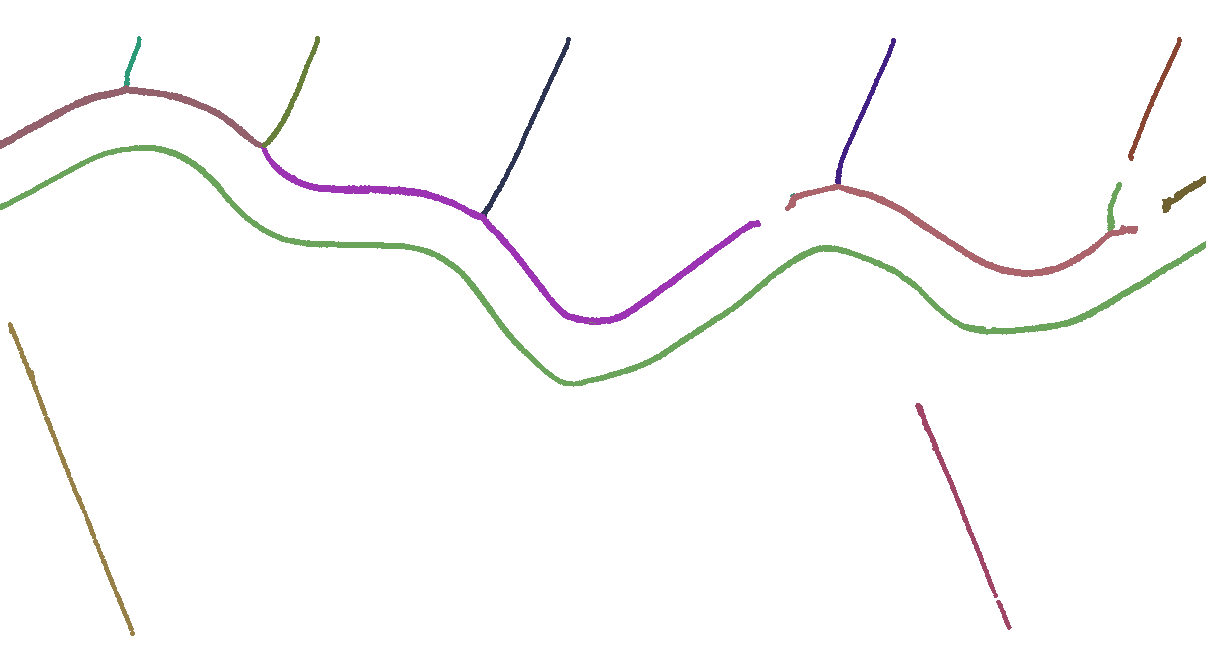
\includegraphics[width=\textwidth,angle=90]{figs/3dmat_plan.png}
		\subcaption{Plan view of exterior skeleton sheets. The medial sheets reflect the structure of the watercourses.}\label{fig:MAT_out_seg_filt}
	\end{subfigure}%
	\caption[MATsegmentation]{Water course detection wiht the 3D MAT. Each distinct medial sheet was assigned a random colour. The surface points are coloured by elevation (yellow = low; blue = high).}
	\label{fig:MATsegmentation}
\end{figure}
Here the bottom edges of the medial sheets are projected to the $xy$ plane to obtain 2D lines that delineate the watercourses.
\citet{Peters18} gives some examples of how the 3D MAT can be used to perform building detection in lidar point clouds.

A second application of the 3D MAT is visibility analysis in point clouds \citep{Peters15}.
Here the difficulty is that point do not have an area and can thus not be used to obstruct visibility rays.
However, the medial balls of the interior MAT do represent the interior volume of objects and can thus be used to obstruct the visibility rays.

% Finally there are some examples of using the 3D MAT for surface reconstruction from points clouds, \ie to obtain a triangulated mesh from a boundary point cloud. 
% This is different from 
% 	\item[Object detection] \citet{Broersen17}
% 	\item[Visibility anlysis] \citet{Peters15}
% \end{description}

\section{Notes and comments}
% Notice that especially the idea of applying the 3D MAT to digital terrain modelling is relatively new and still offers exciting oppurtunities for research.
The Medial Axis Transform was originally introduced in 1967 by Harry Blum, a biologist \citep{Blum67}.

The algorithm to approximate the 2D MAT from the VD is described in detail by \citet{Gold99} and \citet{Gold01}.

\citet{Ma12} introduced the shrinking ball algorithm. \citet{Peters18} explains how to make the algorithm robust so that it can be successfully applied to lidar point cloud inputs and how to obtain a sheet segmentation using a region-growing approach.

%%%%%%%%%%%%%%%%%%%%
%
\section{Exercises}

\begin{enumerate}
  \item laba33
  \item aldkfj
\end{enumerate}
